\section{Introduction}
	This document covers the work done for the project executed in the LPSC course.
	The work has been done by Adrien Balleyguier (with at times help for review from Jonathan Amez-Droz, Dimitri Bavarel and Yann Sierro).\\
	The sources are made available at the following link:
	\begin{center}
		\href{https://github.com/adrien-balleyguier/julia_adrien_balleyguier}{https://github.com/adrien-balleyguier/julia\_adrien\_balleyguier}
	\end{center}
    The document describes the goals and means of the project.
    A last section is dedicated to things that could be added, or modified, with indications about the hows.\\
    For display purpose, schematics are given as annexes.
    Considering the size such schematics can have, they are added in vectorized format.
    Each schematic's purpose is squared in blue.
\section{Description}
    The project goal is to consider a julia set defined by a given constant.
    This set value are to be computed and displayed using VHDL on a \texttt{xc7z012clg485-2} board.
    The realisation contraint adds parallelisation for the computation tasks, allowing to process the complete screen
    faster.\\
    For context, the julia set equation is the complex plan, with each point computed with regards to the equation
    \begin{equation}\label{equ:definition}
        z_{n+1} = z_n^2 + c
    \end{equation}
    Each point coordinates serves as $z_0$ in \eqref{equ:definition}.
    The used constant for this application is $c=-0.123+0.745i$.
    Using and independent application, the results should look like the picture \ref{fig:expected_display}.
    \begin{figure}[H]
        \centering
        
\includegraphics[width=0.6\textwidth]{expected_display.png}
        \caption{Expected display on the HDMI screen with regards to the displayed area and colour.}
        \label{fig:expected_display}
    \end{figure}
    Each colour in \ref{fig:expected_display} indicates the amount of iteration in the $z_n$ sequence before divergence.
    Said divergence occurs when $|z_n| > 2$.
    The points in black indicates points that did not reach divergence after 100 iterations.
\section{Achieved work}
    The achieved work is divided into logical blocks.
    \subsection{Pixel computation}
        A pixel is associated a complex point which serves as $z_0$ for its computation.
        The output reflects the number of iterations required to meet the divergence.\\
        To achieve this, two blocks are implemented:
        \begin{itemize}
            \item compute : charged of computing $z_{n+1}$ and indicating if it diverges (thanks to the norm).
                The block diagram is available in annexe \ref{anx:compute}.
            \item compute\_encapsulate : charged of tracking the amount of iteration for a given point.
                It also tracks the current computing state in the state machine described in figure \ref{fig:compute_state_diagram}.
                The block diagram is available in annexe \ref{anx:compute_encapsulate}.
        \end{itemize}
        To track the computation state, an implicit state machine is used.
        It is implicit because tracked by distinct flags instead of an explicit state.
        This state machine is described in figure \ref{fig:compute_state_diagram}.
        \begin{figure}[H]
            \centering
            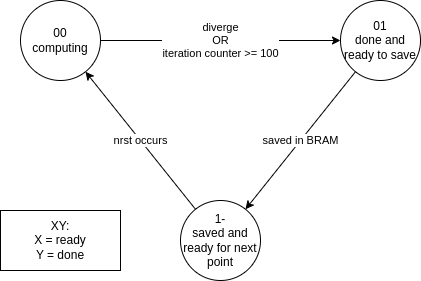
\includegraphics[width=0.6\textwidth]{images/compute_state_diagram.png}
            \caption{State machine describing the computation state for a given computation block}
            \label{fig:compute_state_diagram}
        \end{figure}
    \subsection{Mapping between pixel and complex point}
        One can consider two set of points used throughout the computations:
        \begin{itemize}
            \item Complex points : the displayed set of points
            \item pixel : the actual pixel of the 720x720 screen
        \end{itemize}
        A bijective mapping exists between this two sets and the coordinate\_tracker block is in charge if ensuring such.
        The block will then iterate over the 720x720 points available and computing the corresponding complex point.
        An added flag allows to pause the aforementioned iterations.
        The block diagram is available in annexe \ref{anx:coordinate_tracker}.
    \subsection{BRAM}
        The computation results needs to be written somewhere for the HDMI to read them.
        This read and write can consider their own clock frequencies.
        The BRAM content is NOT changed on a reset.
        The reason is the synthesis time in vivado that took significantly more time.
        The only drawback would be to read data which are not the actual one for a given pixel.
        However the computing speed allows to ignore it as the pixel will receive it's proper value too quickly for
        anyone to notice.
    \subsection{Priority encoder}
        As mentioned the compute bloc will be duplicated to allow for parallel, thus faster, computation.
        When setting a new $z_0$, respectively writing a point to the BRAM, one of the computation block needs to be
        selected.
        Priority encoder allows to do so.
        While not impacting the results nor the resulting computation time, a subtle element is to point out.
        Assigning an index to each computation block, a block with higher index will be used more than the others.
        The reason is that a low index will have to wait for the other block to be saved.
        Should a block with high index compute quickly enough, it will be able to save his results qhile the lower
        index still waits.
\section{Results}
    The results on the screen can be illustrated with the pictures \ref{fig:result_11_22} and \ref{fig:result_00_11}
        \begin{figure}[H]
            \centering
            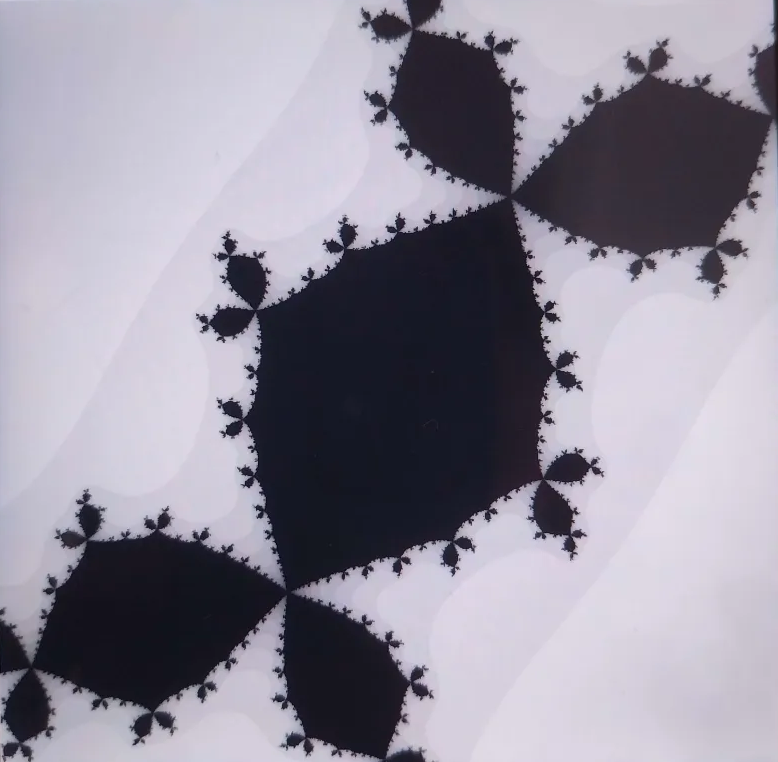
\includegraphics[width=0.8\linewidth]{images/result_11_22.png}
            \caption{Computation results for the bottom left point = (-1, -1) with width = 2 and height = 2}
            \label{fig:result_11_22}
        \end{figure}
        \begin{figure}[H]
            \centering
            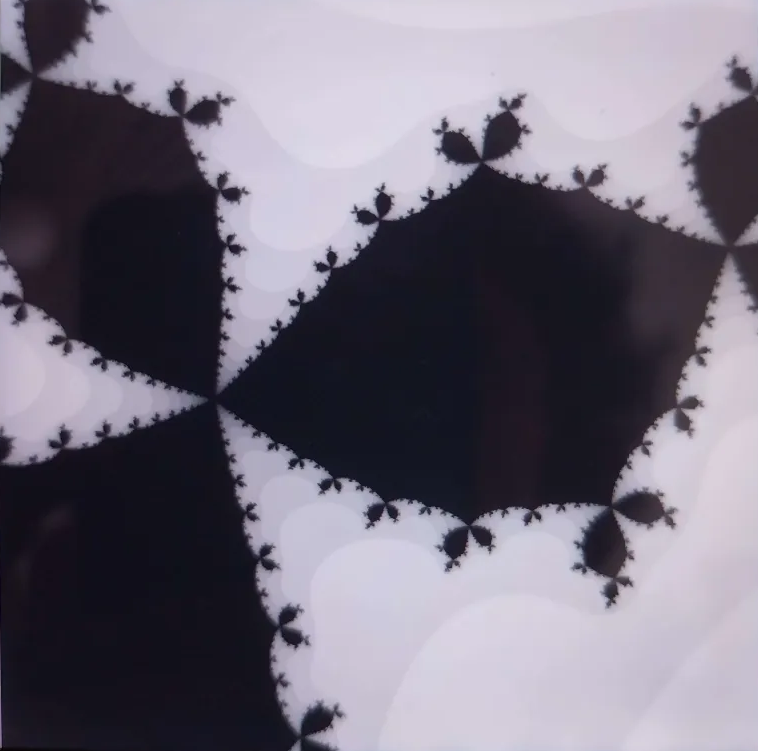
\includegraphics[width=0.8\linewidth]{images/result_00_11.png}
            \caption{Computation results for the bottom left point = (0, 0) with width = 1 and height = 1}
            \label{fig:result_00_11}
        \end{figure}
    The computation time, observed through simulation, are available in the table \ref{tab:result_time}.
    \begin{table}[H]
        \begin{center}
            \begin{tabular}{|c|c|}\hline
                number of compute block in parallel & time [clock ticks]\\\thickhline
                1  & 13138033 \\\hline
                2  & 6569017 \\\hline
                4  & 3445079 \\\hline
                8  & 2161663 \\\hline
                16 & 1703673 \\\hline
            \end{tabular}
            \caption{Number of clock tick required to iterate throught the 720x720 pixels with regards to the amount
                of computation block in parallel. The bottom left point is (0, 0), width = 2 and height = 3}
            \label{tab:result_time}
        \end{center}
    \end{table}
    Plotting this table will lead to the graph available in the figure \ref{fig:time_compute_results}.
    One can point out that the computation time changes according to the power of 2 changes.
    For instance, using 2 blocks will divide the time by 2, 4 blocks will divide the time by 3, ...\\
    The actual number of clock would be a bit higher because of the writing in the BRAM.
    This writing adds a clock tick delay at the end of the computation.
    \begin{figure}[H]
        \centering
        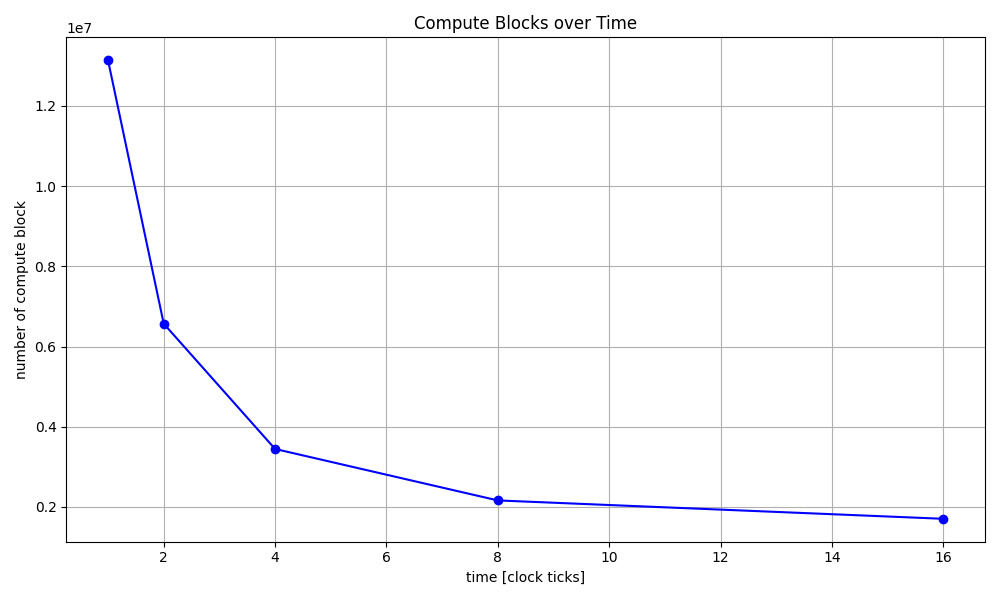
\includegraphics[width=0.8\linewidth]{images/time_compute_results.png}
        \caption{Computation time [clock ticks] with regards to the amount of computation blocks. This results
            have been observed in simulation}
        \label{fig:time_compute_results}
    \end{figure}
    Please consider that a single computation blocks takes up to 9 DSP.
    Considering that the amount of available DSP on the target is 170, this means that we could consider up to 16
    computation block for a deployment.
    However, the other elements consumes someof this DSPs leading to the actual count being lower.
    The number of computation blocks used for the demonstration was 8.\\
    The synthesis of the complete computation blocks is made available in the annexe \ref{anx:complete_synthesis} 
    at the discretion of the block detailed in other annexes.
\section{Feature that could be added}
    Some features would have been implemented should more effort have been available:
    \begin{itemize}
        \item Explicit clock management.
            Thanks to a dedicated PLL, the computation clock could be in total control.
            This would not impact the results
        \item Zoom and moving with button management.
            The board gives access to various buttons.
            One could use them to interact with the display.
            Each button pressing would change the screen variables (first point, width, height) and reset the
            computation block.\\
            Considering the aforementioned computation time, a delay between the pressing and the new display should
            not be observable.
        \item Adding color.
            The current display is in shades of grey (more than 50).
            Allowing the user to select between this and a colorful one could be added thanks to buttons.
            This would only impact the block in charge of sending data to the HDMI.
    \end{itemize}
\section{Personal feedback on the work}
    The project was interesting and challenging at times.
    I started the semestre with only memory of VHDL from 5 years ago and this has added to the challenge.
    In the end I would have been able to implement some of the feature listed above if I was more fluent in VHDL upon
    starting.\\
    Obviously I leave some elements in the code with some tinkering.
    Should I start again I would clean them up, starting with the compute encapsulation.
%keep for proper page numbering
\label{page:end_redaction}
